\documentclass{article}

\usepackage{fancyhdr} % Required for custom headers
\usepackage{lastpage} % Required to determine the last page for the footer
\usepackage{extramarks} % Required for headers and footers
\usepackage[usenames,dvipsnames]{color} % Required for custom colors
\usepackage{graphicx} % Required to insert images
\usepackage{listings} % Required for insertion of code
\usepackage{courier} % Required for the courier font
\usepackage{lipsum} % Used for inserting dummy 'Lorem ipsum' text into the template
\usepackage{hyperref}
\usepackage{multirow}
\usepackage{tabularx}
\usepackage{framed}
\usepackage{longtable}
\usepackage{listings}
\usepackage{subfigure}
\usepackage{afterpage}
\usepackage{amsmath,amssymb}            
\usepackage{rotating}  
\usepackage{fancyhdr}
\usepackage{graphicx}
\usepackage{amsthm}
\usepackage[scriptsize]{caption} 
\hyphenation{a-gen-tiz-za-zio-ne}
% Margins
\topmargin=-0.45in
\evensidemargin=0in
\oddsidemargin=0in
\textwidth=6.5in
\textheight=9.0in
\headsep=0.25in

\linespread{1.1} % Line spacing

\lstset{
  numbers=left,
  stepnumber=5,    
  firstnumber=1,
  numberfirstline=true
}

% Set up the header and footer
\pagestyle{fancy}
\lhead{\hmwkAuthorName} % Top left header
\chead{\hmwkClass\ (\hmwkClassInstructor\ \hmwkClassTime): \hmwkTitle} % Top center head
\rhead{\firstxmark} % Top right header
\lfoot{\lastxmark} % Bottom left footer
\cfoot{} % Bottom center footer
\rfoot{Page\ \thepage\ of\ \protect\pageref{LastPage}} % Bottom right footer
\renewcommand\headrulewidth{0.4pt} % Size of the header rule
\renewcommand\footrulewidth{0.4pt} % Size of the footer rule

\setlength\parindent{0pt} % Removes all indentation from paragraphs

\usepackage{listings}
\usepackage{color}

\definecolor{dkgreen}{rgb}{0,0.6,0}
\definecolor{gray}{rgb}{0.5,0.5,0.5}
\definecolor{mauve}{rgb}{0.58,0,0.82}

\lstset{frame=tb,
  language=Java,
  aboveskip=3mm,
  belowskip=3mm,
  showstringspaces=false,
  columns=flexible,
  basicstyle={\small\ttfamily},
  numbers=none,
  numberstyle=\tiny\color{gray},
  keywordstyle=\color{blue},
  commentstyle=\color{dkgreen},
  stringstyle=\color{mauve},
  breaklines=true,
  breakatwhitespace=true
  tabsize=3
}

%----------------------------------------------------------------------------------------
%	DOCUMENT STRUCTURE COMMANDS
%	Skip this unless you know what you're doing
%----------------------------------------------------------------------------------------

% Header and footer for when a page split occurs within a problem environment
\newcommand{\enterProblemHeader}[1]{
\nobreak\extramarks{#1}{#1 continued on next page\ldots}\nobreak
\nobreak\extramarks{#1 (continued)}{#1 continued on next page\ldots}\nobreak
}

% Header and footer for when a page split occurs between problem environments
\newcommand{\exitProblemHeader}[1]{
\nobreak\extramarks{#1 (continued)}{#1 continued on next page\ldots}\nobreak
\nobreak\extramarks{#1}{}\nobreak
}


%----------------------------------------------------------------------------------------
%	NAME AND CLASS SECTION
%----------------------------------------------------------------------------------------

\newcommand{\hmwkTitle}{Concorrenza} % Assignment title
\newcommand{\hmwkDueDate}{Mercoled\`i,\ Maggio 11,\ 2016} % Due date
\newcommand{\hmwkClass}{Ingegneria del Software 1} % Course/class
\newcommand{\hmwkClassTime}{} % Class/lecture time
\newcommand{\hmwkClassInstructor}{Claudio Menghi, Alessandro Rizzi} % Teacher/lecturer
\newcommand{\hmwkAuthorName}{} % Your name

%----------------------------------------------------------------------------------------
%	TITLE PAGE
%----------------------------------------------------------------------------------------
\newcounter{EsercizioCounter}
 \setcounter{EsercizioCounter}{1}


\newcommand{\Esercizio}[1]{
%\setlength{\fboxsep}{2pt}
\fbox{
   
  \parbox[t][]{\textwidth}{
   \vspace{2ex}
   \textbf{Esercizio \arabic{EsercizioCounter}}: #1
    \vspace{2ex}
    \refstepcounter{EsercizioCounter}
  }
}
}



%----------------------------------------------------------------------------------------

\begin{document}

\maketitle

%----------------------------------------------------------------------------------------
%	TABLE OF CONTENTS
%----------------------------------------------------------------------------------------

%\setcounter{tocdepth}{1} % Uncomment this line if you don't want subsections listed in the ToC

\newpage
\tableofcontents
\newpage



\section{Sistemi concorrenti}
I computer odierni possono eseguire pi\`u di un processo alla volta.  Anche un singolo processo pu\`o eseguire pi\`u operazioni in contemporanea. La piattaforma Java fornisce un supporto per lo sviluppo di sistemi concorrenti. Tale supporto \`e contenuto nel package \emph{java.util.concurrent}.

\subsection{Processi e thread}
In un sistema concorrente ci sono due diversi tipi di elementi che possono essere eseguiti: \emph{processi} e \emph{threads}. 
\begin{itemize}
\item \emph{processi} sono ambienti di esecuzione self-contained, hanno un set di risorse private a run-time e un loro \emph{spazio in memoria}. Per comunicare pi\`u processi hanno bisogno di ``tecniche complesse" e.g., sockets.
\item \emph{threads} sono ``processi a basso costo" richiedono meno risorse, esistono all'interno di \emph{un} processo e condividono le risorse, i file etc. Questo rende molto efficiente la comunicazione tra i threads ma sotto un certo aspetto pi\`u problematica (come vedremo in seguito). Nota ogni processo \`e associato ad almeno un thread principale che pu\`o chiamare pi\`u thread secondari. C'e' \emph{sempre} almeno un thread all'interno della vostra applicatione. Il \emph{main} thread viene associato al metodo main dell'applicazione. 
\end{itemize}

\subsubsection{Problemi nell'utilizzo dei thread}
\begin{itemize}
\item \emph{interferenze}: sono dovuti al fatto che diversi thread lavorano in parallelo sugli stessi dati
\item \emph{liveness} un applicazione viene eseguita entro accettabili vincoli di tempo, sue sottopropriet\`a sono:
\begin{itemize}
\item \emph{deadlock}: due thread sono bloccati uno in attesa dell'altro;
\item \emph{starvation}: un thread ha difficolt\`a a prendere la risorsa, gli altri thread spendono molto tempo o hanno uno scheduler che li aiuta;
\item \emph{livelock}: genera una sequenza ciclica di operazioni inutili.
\end{itemize}
\end{itemize}

\subsection{Thread in Java}
Ogni thread \`e associato a un istanza della classe Thread. Ci sono due strategie per utilizzare i thread nella vostra applicazione:
\begin{itemize}
\item controllare direttamente la creazione e la gestione dei thread all'interno della vostra applicazione
\item separare la \emph{logica} di gestione dei thread dal resto della vostra applicazione (vedi in seguito executors).
\end{itemize}


\subsubsection{Stati di un thread}
In un determinato istante temporale ogni thread si trova inuno stato specifico
\begin{itemize}
\item \emph{born} \`e lo stato che viene raggiunto dopo che  viene eseguita l'istruzione 
\begin{lstlisting}[language=Java]
Thread t=new Thread(Runnable target, String name);
\end{lstlisting}
L'oggetto di tipo thread \`e creato (come un altro oggetto) ma il thread non \`e  ``ready"
\item \emph{ready} viene raggiunto quando viene invocato il metodo \texttt{start} di thread. In questo stato il thread non st\`a eseguendo nulla, \`e solo pronto ad eseguire il codice.
\item \emph{running} viene raggiunto quando effettivamente il codice all'interno di run viene eseguito. 
\item \emph{sleep} quando viene invocato il metodo sleep sul thread. Non c'\`e nessuna garanzia che il thread entra nello stato sleep esattamente nel momento in cui il metodo viene invocato. 
\item \emph{waiting} un thread viene messo in questo stato quando viene invocato il metodo \texttt{wait}
\item \emph{blocked} il thread \`e bloccato quando attende un particolare lock monitorato o di accedere a un metodo synchronized. 
\item \emph{dead} quando il thread \`e terminato. Non \`e pi\`u possibile invocare il metodo \texttt{start} su un thread terminato.
\end{itemize}

\begin{figure}[h!]
  \centering
    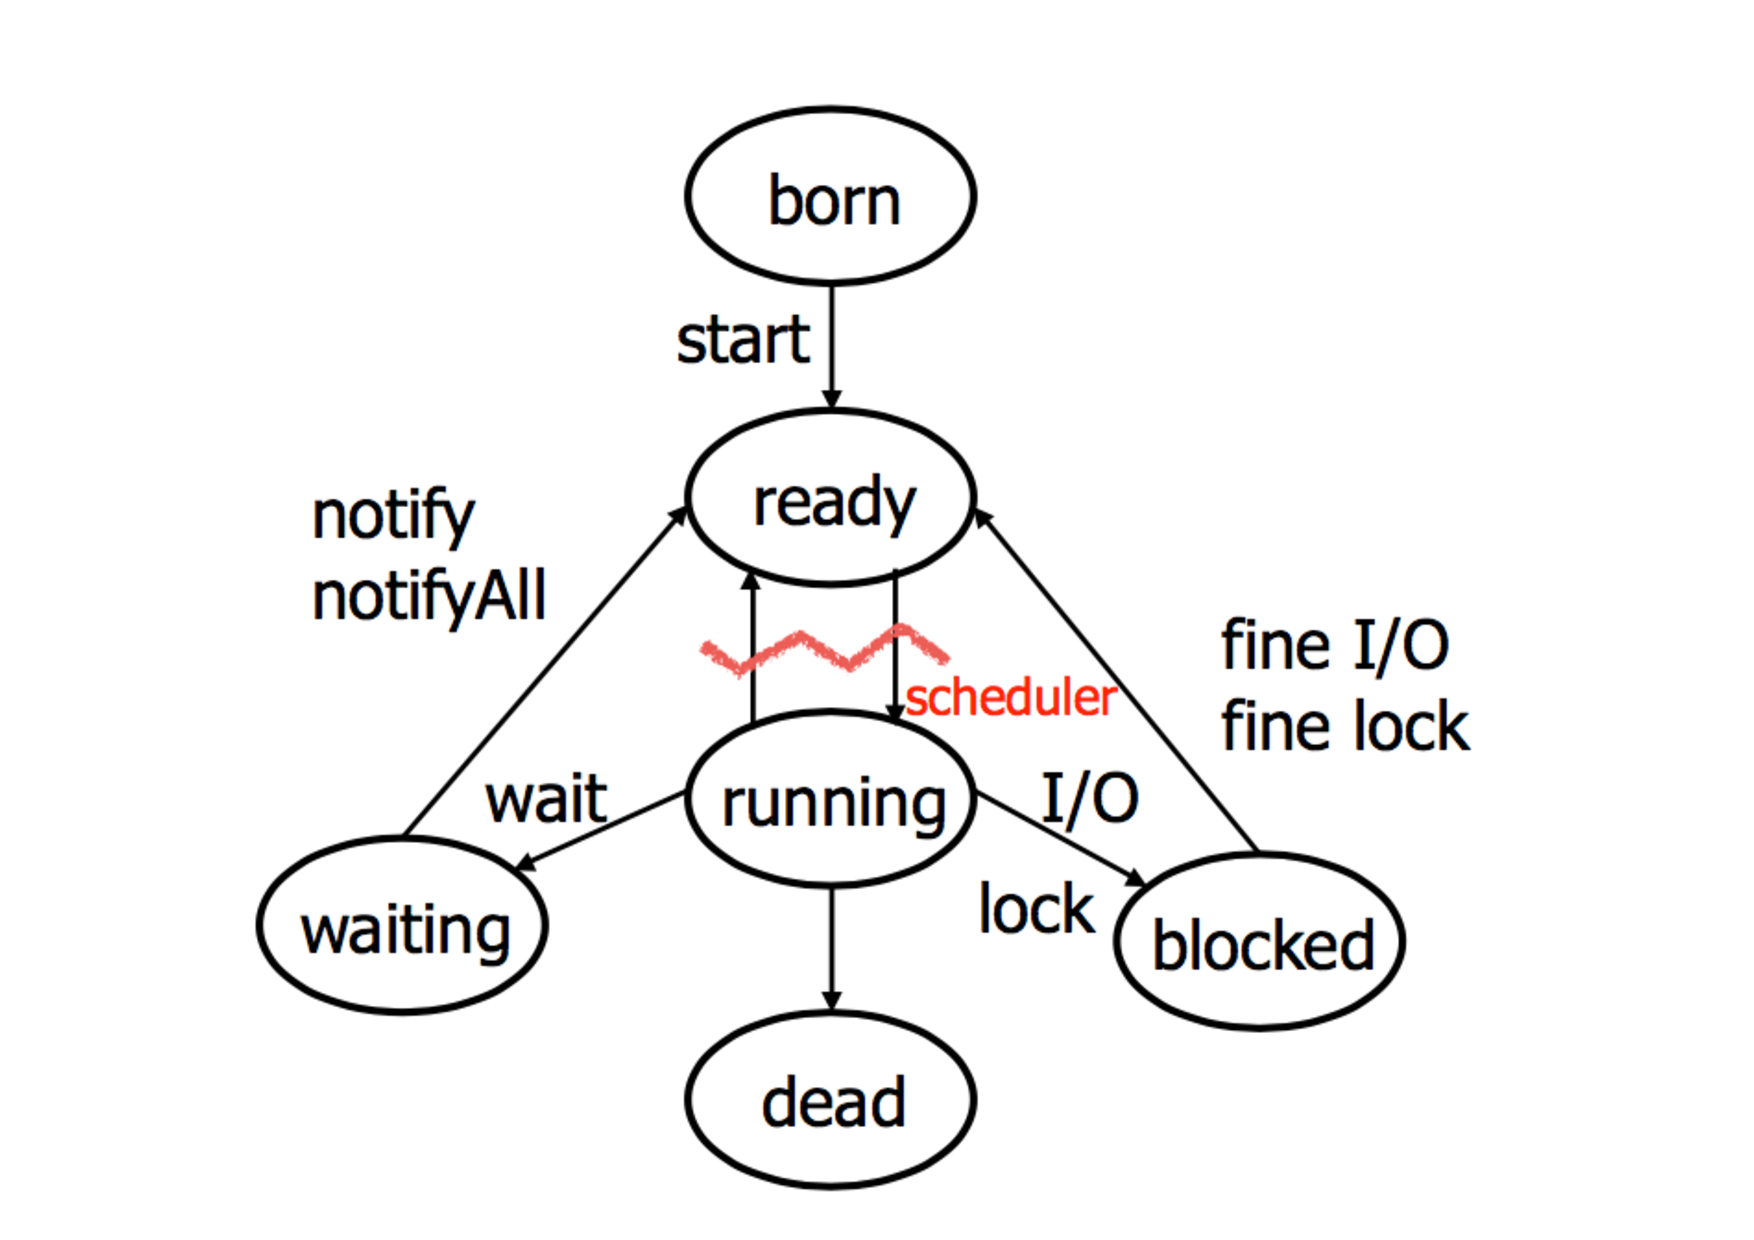
\includegraphics[width=0.8\textwidth]{stati.pdf}
\end{figure}

\subsubsection{Creazione di un thread}
Ci sono due strategie per creare un thread:
\begin{itemize}
\item \emph{creare un oggetto runnabile}: basta implementare l'interfaccia \emph{Runnable} che ci forza a implementare il metodo \emph{run} che contiene il codice eseguito dal thread. Per esempio nel seguente la classe \texttt{HelloRunnable} implementa \texttt{Runnable}.  
\begin{lstlisting}[language=Java]
public class HelloRunnable implements Runnable {

    public void run() {
        System.out.println("Hello from a thread!");
    }
}
\end{lstlisting}
Per creare il thread \`e sufficiente istanziare un oggetto di classe \texttt{Thread} a cui viene passato il riferimento all'oggetto runnabile. 
\begin{lstlisting}[language=Java]
Thread t=new Thread(new HelloRunnable())
\end{lstlisting}
L'istruzione \texttt{Thread t=new Thread(new HelloRunnable());} istanzia una nuova variabile \texttt{t} di tipo thread.
Al costruttore della classe \texttt{Thread} viene passato un oggetto runnabile, nel caso specifico una nuova istanza della classe \texttt{HelloRunnable}. Per eseguire il thread \`e necessario chiamare il metodo \texttt{start} (il quale al suo interno chiama il vostro metodo \texttt{run}).
\begin{lstlisting}[language=Java]
t.start();
\end{lstlisting}

\item \emph{estendere la classe Thread}: la classe thread ha un implementazione di default del metodo \texttt{run} che non fa nulla. \`E necessario overridare il metodo \texttt{run} della classe \texttt{Thread}. Attenzione, se la vostra classe estende \texttt{Thread} non pu\`o estendere un altra classe. In realt\`a quando diciamo che la nostra classe estende Thread stiamo dicendo che la nostra classe \`e una versione ``customizzata" della classe Thread in Java, ovvero che la nostra classe \`e un Thread. Per questo \`e buona prassi non utilizzare l'estensione solo per overridare il metodo \texttt{run}.
\begin{lstlisting}[language=Java]
public class HelloRunnable extend Thread {

    public void run() {
        System.out.println("Hello from a thread!");
    }

    public static void main(String args[]) {
        HelloRunnable t=new HelloRunnable();
        t.start();
    }
}
\end{lstlisting}
\end{itemize}

La classe \texttt{Thread} offre una serie di metodi statici (e non) utili nella gestione dei threads (vedi la Javadoc corrispondente).

Interessante \`e anche la possibilit\`a di identificare il thread per mezzo di un nome utilizzando l'apposito costruttore (questo ci consente di identificarlo agevolmente)
\begin{lstlisting}[language=Java]
Thread t=new Thread(Runnable target, String name);
\end{lstlisting}

 o raggruppare dei threads (per esempio raggruppare dei threads che svolgono delle attivit\`a simili.
 \begin{lstlisting}[language=Java]
Thread t=new Thread(ThreadGroup threadGroup, Runnable target, String name);
\end{lstlisting}





\subsection{Interferenze}
I thread comunicano tra loro principalmente mediante l'accesso ad attributi degli oggetti che condividono. Questa forma di comunicazione \`e estremamente efficiente ma rende possibili vari errori: i pi\`u comuni sono le interferenze. Le interferenze avvengono quando pi\`u thread accedono in meniera concorrente alle medesime risorse. Per esempio vedi l'esercizio 2. Per evitare questi problemi dobbiamo garantire che l'accesso a determinate porzioni di codice avvenga in maniera atomica, non sia consentito a due thread distinti l'accesso a porzioni di codice che possono generare inconsistenze.

Ci sono 2 possibili modi per prevenire questi problemi:
\begin{itemize}
\item \emph{metodi sincronizzati}: \`e sufficiente aggiungere la keyword \texttt{synchronized} nella dichiarazione del metodo
\begin{lstlisting}[language=Java]
public synchronized void increment();
\end{lstlisting}
Ad ogni oggetto viene associato un \texttt{lock} intrinseco che svolge un ruolo primario nella sincronizzazione. Prima di eseguire un metodo \texttt{sinchronized} un thread deve acquisire il lock intrinseco dell'\textbf{oggetto} e rilasciarlo quando ha finito.
\item \emph{statements sincronizzati}: a differenza dei metodi sincronizzati, gli statement sincronizzati richiedono di specificare l'oggetto su cui di desidera avere il lock intrinseco. Per esempio, nel metodo \texttt{addName}
\begin{lstlisting}[language=Java]
public void addName(String name) {
    synchronized(this) {
        lastName = name;
        nameCount++;
    }
    nameList.add(name);
}
\end{lstlisting}
il lock viene acquisito sull'oggetto corrente e viene tenuto per la durata delle due istruzioni \texttt{lastName = name;} e \texttt{nameCount++;}. Attenzione, l'invocazione di altri metodi all'interno di un blocco sincronizzato potrebbe causare problemi di \texttt{liveness}. L'utilizzo di statement sincronizzati consente di avere un livello pi\`u granulare nella gestire la sincronizzazione.
\end{itemize}


\subsubsection{Interazione tra threads}
I threads molto spesso devono coordinare le loro azioni. Il caso del \texttt{guarded block} \`e uno dei casi pi\`u comuni. Una guarded block \`e una condizione che deve essere vera prima che l'esecuzione di un blocco possa procedere. Una prima procedura consiste nell'eseguire un \texttt{while} infinito finch\`e una condizione non \`e verificata. Questa scelta \`e molto inefficiente. Utilizziamo un metodo pi\`u furbo: ricorriamo al metodo wait della classe Thread.
\begin{itemize}
\item \emph{wait}: sospende il thread corrente. Il thread non viene risvegliato finch\`e non riceve una notifica.
\end{itemize}
Due metodi possono essere utilizzati per svegliare i thread
\begin{itemize}
\item \emph{notifyAll}: manda una notifica a \emph{tutti} i thread che sono in sleep in attesa di quel lock. I thread corrispondenti si svegliano.
\item \emph{notify}: sveglia non deterministicamente un singolo thread tra tutti quelli in attesa sulla risorsa.
\end{itemize}

\subsection{Concorrenza di alto livello}

\subsubsection{Lock Objects}
Fino ad ora abbiamo utilizzato il lock intrinseco di Java per specificare come i thread devono interagire. Questo lock \`e facile da utilizzare ma ha molte limitazioni. I lock object forniscono degli strumenti di pi\`u alto livello per gestire la sincronizzazione, per esempio \`e possibile specificare condizioni sull'esecuzione dei threads mediante l'interfaccia \texttt{Condition}. Per esempio,  i lock objects forniscono il metodo
\begin{itemize}
\item \texttt{tryLock}  prova a prendere il lock,  se non lo ottiene continua l'esecuzione invece di mandare il thread in wait
\item \texttt{lockInterruptibly} consente il ritiro di un thread se un altro thread manda un interrupt prima che il lock sia acquisito.
\end{itemize}

\subsubsection{Esecutori}
Negli esempi precedenti c'\`e una forte relazione tra task e thread, dal momento che il task deve essere un \texttt{Runnable} ed istanziato mediante un oggetto thread. \`E possibile tenere i concetti distinti mediante 
\begin{itemize}
\item \texttt{Executor}
\item \texttt{Thread Pools}
\item \texttt{Fork and Join}
\end{itemize}

\textbf{Executors}\\
ci sono 3 diverse interfacce che consentono di gestire i thread
\begin{itemize}
\item Executor: interfaccia che permette di lanciare nuovi task. Le sue implementazioni usano dei thread pools che consentono di riutilizzare dei thread invece di crearli da campo. Un elemento di tipo executor offre il metodo \texttt{execute(Runnable command)} che consente di eseguire un elemento runnable. 
\item ExecutorService: aggiunge nuove features che consentono di gestire il ciclo vita dei thread. Permettono di utilizzare \texttt{Callable} object invece di oggetti runnabili. I callable object solitamente ritornano un valore. ExecutorService \`e un interfaccia che estende \texttt{Executor} e fornisce metodi quali \texttt{submit(Runnable task)} che submitta un task per l'esecuzione o \texttt{shutdown} il quale inizia lo spegnimento (nuovi task non sono accettati quelli gi\`a in coda sono finiti.
\item ScheduledExecutorServece: interfaccia che permette di specificare informazioni addizionali come la politica di scheduling da utilizzare nella gestione dei vari threads.
\end{itemize}

\textbf{Thread Pools}
Sono utilizzati all'interno di maggior parte degli executors. Sono creati per \emph{minimizzare} l'overhead richiesto alla creazione dei threads, visto che la gestione dei threads richiede un significativo quantitativo di memoria. In genere forniscono un insieme (\emph{pool}) di threads gi\`a preistanziato o riusano i threads terminati (invece di crearli da zero ogni volta).

Per creare un Executor \`e possibile utilizzare i metodi statici contenuti all'interno della classe \texttt{Executors}. Per esempio, \texttt{Executors.newFixedThreadPool(int nThreads)} restituisce un thread pool con un numero di thread predefiniti. In particolare, potrebbero essere utili:
\begin{itemize}
\item SingleThreadExecutor: esegue un solo task alla volta
\item FixedThreadPool: esegue un numero fissato di task in parallelo
\item CachedThreadPool: esegue un numero illimitato di task in parallelo
\item ScheduledThreadPool: permette di programmare l'esecuzione dei task
\end{itemize}

\subsection{Collezioni}
La maggior parte delle collezioni e mappe che abbiamo visto finora non sono thread-safe. Ovviamente le versioni thread safe hanno prestazioni peggiori. Per ottenere una lista sincronizzata \`e possibile per esempio utilizzare il metodo statico \texttt{Collections.synchronizedList(List<T> list)} di \texttt{Collections}. Interessanti sono anche le classi \texttt{CopyOnWriteArrayList} e simili, utili quando non si vuole rendere sincrona l'operazione di iterazione ma solo la modifica della lista. Queste classi sono contenute all'interno del package \texttt{java.util.concurrent}.

\subsection{Variabili atomiche}
Il package java.util.atomic definisce classi che supportano operazioni atomiche su singole variabili per esempio \texttt{AtomicBoolean}.
\begin{itemize}
\item Esse posseggono tutti i metodi (getter e setter) delle classi corrispondenti (Boolean) ma l'esecuzione di ciascuna operazione avviene in maniera atomica.
\item E' disponibile anche l'operazione atomica \texttt{compareAndSet}
\end{itemize} 

\section{Esercizi}

\subsection{Basic: tartaruga vs coniglio}
\Esercizio{
Implementare una gara di corsa tra una tartaruga e un coniglio. La tartaruga e il coniglio proseguono a velocit\`a costante e differente (La tartaruga \`e pi\`u lenta).  Una volta arrivati al traguardo, la tartaruga e il coniglio stampano il messaggio arrivato! Chi arriva prima?
}

Bench\`e la tartaruga sia pi\`u lenta del coniglio, e ogni volta esegue dei passi pi\`u piccoli non abbiamo alcuna garanzia relativa al comportamento dello scheduler. Lo scheduler potrebbe dedicare pi\`u tempo al thread tartaruga consentendogli di arrivare prima al traguardo. \emph{In generale \`e bene non effettuare nessuna assunzione sul comportamento dello scheduler.}


\begin{lstlisting}[language=Java]
package race;

public class Animale implements Runnable {

	private int posizione;
	private Race race;
	private int lunghezzaPasso;

	public Animale(Race race, int lunghezzaPasso) {
		this.race = race;
		this.posizione = 0;
		this.lunghezzaPasso = lunghezzaPasso;
	}

	@Override
	public void run() {
		boolean arrivato=false;
		while (!arrivato) {

			posizione = posizione + lunghezzaPasso;
			if (posizione > this.race.getDistanza()) {
				System.out.println("Sono il thread: "
						+ Thread.currentThread().getName() + " sono arrivato");
				arrivato=true;
			} else {
				System.out.println("Sono il thread: "
						+ Thread.currentThread().getName() + " posizione "
						+ this.posizione);
			}

		}
	}
}
\end{lstlisting}

\begin{lstlisting}[language=Java]
public class Race {
	
	private int distanza;
	private static final int CONIGLIO_LUNGHEZZA_PASSO=5;
	private static final int TARTARUGA_LUNGHEZZA_PASSO=4;
	
	public Race(int distanza){
		this.distanza=distanza;
	}
	
	public int getDistanza(){
		return this.distanza;
	}
	
	public static void main(String[] args) throws InterruptedException {
		Race race=new Race(100);
		Thread coniglio=new Thread(new Animale(race,  CONIGLIO_LUNGHEZZA_PASSO), "CONIGLIO");
		Thread tartaruga=new Thread(new Animale(race,  TARTARUGA_LUNGHEZZA_PASSO), "TARTARUGA");
		coniglio.start();
		tartaruga.start();
	}
}
\end{lstlisting}


\subsection{Sleep: tartaruga vs coniglio}
\Esercizio{
Sia la tartaruga che il coniglio, dopo ogni passo eseguono una pennichella di un tempo prefissato.
}
Attenzione!!! Quando viene invocato il metodo sleep sul thread, non c'\`e nessuna garanzia che il thread entra nello stato sleep esattamente nel momento in cui il metodo viene invocato.

\begin{lstlisting}[language=Java]
package race;

public class Animale implements Runnable {

	private int posizione;
	private Race race;
	private int lunghezzaPasso;
	
	private int pauseTime;

	public Animale(Race race, int lunghezzaPasso, int pauseTime) {
		this.race = race;
		this.posizione = 0;
		this.lunghezzaPasso = lunghezzaPasso;
		this.pauseTime=pauseTime;
	}

	@Override
	public void run() {
		boolean arrivato=false;
		while (!arrivato) {
			try {
				Thread.sleep(this.pauseTime);
			} catch (InterruptedException e) {
				// TODO Auto-generated catch block
				e.printStackTrace();
			}
			posizione = posizione + lunghezzaPasso;
			if (posizione > this.race.getDistanza()) {
				System.out.println("Sono il thread: "
						+ Thread.currentThread().getName() + " sono arrivato");
				arrivato=true;
			} else {
				System.out.println("Sono il thread: "
						+ Thread.currentThread().getName() + " posizione "
						+ this.posizione);
			}

		}
	}
}
\end{lstlisting}

\begin{lstlisting}[language=Java]
public class Race {
	
	private int distanza;
	private static final int CONIGLIO_PAUSE_TIME=2000;
	private static final int CONIGLIO_LUNGHEZZA_PASSO=5;
	private static final int TARTARUGA_PAUSE_TIME=500;
	private static final int TARTARUGA_LUNGHEZZA_PASSO=4;
	
	public Race(int distanza){
		this.distanza=distanza;
	}
	
	public int getDistanza(){
		return this.distanza;
	}
	
	public static void main(String[] args) throws InterruptedException {
		Race race=new Race(100);
		Thread coniglio=new Thread(new Animale(race, CONIGLIO_LUNGHEZZA_PASSO, CONIGLIO_PAUSE_TIME), "CONIGLIO");
		Thread tartaruga=new Thread(new Animale(race,  TARTARUGA_LUNGHEZZA_PASSO, TARTARUGA_LUNGHEZZA_PASSO), "TARTARUGA");
		coniglio.start();
		tartaruga.start();
	}
}
\end{lstlisting}

\subsection{Join: tartaruga vs coniglio}
\Esercizio{
Il main thread deve far partire la tartaruga solamente dopo che il coniglio \`e arrivato
}
\begin{lstlisting}[language=Java]
package race;

public class Animale implements Runnable {

	private int posizione;
	private Race race;
	private int lunghezzaPasso;
	
	private int pauseTime;

	public Animale(Race race, int lunghezzaPasso, int pauseTime) {
		this.race = race;
		this.posizione = 0;
		this.lunghezzaPasso = lunghezzaPasso;
		this.pauseTime=pauseTime;
	}

	@Override
	public void run() {
		boolean arrivato=false;
		while (!arrivato) {
			try {
				Thread.sleep(this.pauseTime);
			} catch (InterruptedException e) {
				// TODO Auto-generated catch block
				e.printStackTrace();
			}
			
			posizione = posizione + lunghezzaPasso;
			if (posizione > this.race.getDistanza()) {
				System.out.println("Sono il thread: "
						+ Thread.currentThread().getName() + " sono arrivato");
				arrivato=true;
			} else {
				System.out.println("Sono il thread: "
						+ Thread.currentThread().getName() + " posizione "
						+ this.posizione);
			}
		}
	}
}
\end{lstlisting}

\begin{lstlisting}[language=Java]
package race;

public class Race {
	
	private int distanza;
	private static final int CONIGLIO_PAUSE_TIME=2000;
	private static final int CONIGLIO_LUNGHEZZA_PASSO=5;
	private static final int TARTARUGA_PAUSE_TIME=500;
	private static final int TARTARUGA_LUNGHEZZA_PASSO=4;
	
	public Race(int distanza){
		this.distanza=distanza;
	}
	
	public int getDistanza(){
		return this.distanza;
	}
	
	public static void main(String[] args) throws InterruptedException {
		Race race=new Race(100);
		Thread coniglio=new Thread(new Animale(race, CONIGLIO_LUNGHEZZA_PASSO, CONIGLIO_PAUSE_TIME), "CONIGLIO");
		Thread tartaruga=new Thread(new Animale(race,  TARTARUGA_LUNGHEZZA_PASSO, TARTARUGA_LUNGHEZZA_PASSO), "TARTARUGA");
		coniglio.start();
		coniglio.join();
		// devi attendere finch`e il coniglio non finisce prima che la tartaruga parta
		tartaruga.start();
	}
}
\end{lstlisting}




\subsection{Interferenze: contatore}
\Esercizio{
Il contatore \`e progettato per incrementare e sottrarre una unit\`a da \texttt{c}. Tuttavia il contatore pu\`o essere utilizzato da threads multipli.
\`E corretto?
} 
\begin{lstlisting}[language=Java]
class Counter {
    private int c = 0;

    public void increment() {
        c++;
    }

    public void decrement() {
        c--;
    }

    public int value() {
        return c;
    }
}
\end{lstlisting}
In questo caso potrebbe esservi un problema di interferenza, che si verifica quando i due threads sono interleaved. Anche se le operazioni \texttt{c++;} e \texttt{c--;} sono singoli statements \`e possibile che vengano tradotti in pi\`u istruzioni macchina, per esempio prendi il valore corrente di c, incrementa il valore di 1 e rimetti il calore in c.



Supponiamo che i due thread \texttt{A} e \texttt{B} invocano un incremento e un decremento sul contatore nello stesso momento. Considerando il loro interleaving \`e possibile ottenere
\begin{itemize}
\item Thread A prendi c
\item Thread B prendi c
\item Thread A incrementa il valore 1
\item Thread B decrementa il valore -1
\item Thread A memorizza il valore in C ( c=1)
\item Thread B memorizza il valore in C (c=-1)
\end{itemize}
A questo punto il valore computato dal thread A viene perso: il risultato finale \`e indipendente da tutto il lavoro che si \`e fatto A. 

\begin{lstlisting}[language=Java]
public class SynchronizedCounter {
    private int c = 0;

    public synchronized void increment() {
        c++;
    }

    public synchronized void decrement() {
        c--;
    }

    public synchronized int value() {
        return c;
    }
}
\end{lstlisting}
In questa versione 
\begin{itemize}
\item non \`e possibile eseguire due metodi synchronized in parallelo: quando un thread sta eseguendo un metodo synchronized tutti gli altri thread che invocano metodi synchronized (sullo stesso oggetto) sono sospesi finch\`e il thread non ha finito di eseguire il  metodo. Il thread che st\`a eseguendo il metodo synchronized ha il lock sull'oggetto.
\item quando il metodo synchronized viene lasciato, vengono automaticamente risvegliati i thread in attesa di quell'oggetto. 
\end{itemize}
\emph{In genere se un oggetto \`e visibile a pi\`u di un thread tutti i metodi che leggono e scrivono le variabili di quell'oggetto devono essere \texttt{synchronized}, con l'eccezione di attributi \texttt{final}}.




\subsection{Interferenze: sala da ballo}
\Esercizio{
Modellizzare una sala da ballo. All'interno della sala da ballo ci sono delle Dame, ognuna dell quali pu\`o essere in due stati: \texttt{IN\_COPPIA} o \texttt{SENZA\_UOMO}. Un cavaliere sceglie una dama dalla sala e le chiede di ballare. Se la dama ha gi\`a un cavaliere, ritorna \texttt{false}, altrimenti la dama \`e libera di ritornare \texttt{true} o \texttt{false} in relazione al gradimento per il cavaliere. Dopo aver eseguito un ballo (pi\`u o meno lungo) il cavaliere rilascia la dama.}

\begin{lstlisting}[language=Java]
import java.util.ArrayList;
import java.util.Collections;
import java.util.List;
import java.util.Random;

public class Cavaliere implements Runnable {

	private final SalaBallo salaBallo;

	private final Random random;

	private final String id;

	public Cavaliere(String id, Random random, SalaBallo salaBallo) {
		this.id = id;
		this.random = random;
		this.salaBallo = salaBallo;
	}

	private void iterate() {
		// si aggira guardingo alla ricerca della preda
		List<Dama> dame=new ArrayList<Dama>(this.salaBallo.getDame());
		try {
			Thread.sleep(5000 * random.nextInt(5));
		} catch (InterruptedException e) {
			e.printStackTrace();
		}
		Collections.shuffle(dame);
		Dama d=dame.get(0);
		if(d.rispondi()){
			try {
				System.out.println("Sono "+this.id+" la mia dama e' "+d.getName());
				Thread.sleep(5000 * random.nextInt(5));
				
			} catch (InterruptedException e) {
				e.printStackTrace();
			}
			d.rilascia();
			System.out.println("Sono "+this.id+" ho lasciato "+d.getName());
		}
		else{
			System.out.println("Sono "+this.id+" sono stato rifiutato da "+d.getName());
			
		}
	}
	@Override
	public void run() {
		while (true) {
			iterate();
		}
	}
}
\end{lstlisting}

\begin{lstlisting}[language=Java]
import java.util.Random;


public class Dama {
	/**
	 * contiene il nome della dama
	 */
	private final String name;
	
	/**
	 * contiene lo stato della dama (LIBERA o IN_COPPIA)
	 */
	private Stato stato;
	/**
	 * contiene un generatore random, che modellizza
	 * i gusti della donna in fatto di uomini
	 */
	private Random random;
	
	/**
	 * crea una dama con un deteminato nome
	 * @param name il nome della dama
	 * @param random un generatore utilizzato nella scelta dell'uomo
	 */
	public Dama(String name, Random random){
		this.name=name;
		this.random=random;
		this.stato=Stato.LIBERA;
	}

	/**
	 * ritorna il nome della dama
	 * @return il nome della dama
	 */
	public String getName() {
		return name;
	}
	
	/**
	 * viene invocata dall'uomo dopo un numero di balli
	 * consente di rilasciare la dama
	 */
	public synchronized void rilascia(){
		this.stato=Stato.LIBERA;
	}
	
	/**
	 * ritorna una risposta a una richiesta di Ballo
	 * @return una risposta a una richiesta di ballo. Se la dama e' occupata
	 * la risposta e' no. Altrimenti dipende dal suo gradimento per il cavaliere
	 */
	public synchronized boolean rispondi(){
		if(this.stato==Stato.IN_COPPIA){
			return false;
		}
		boolean result=this.random.nextBoolean();
		if(result){
			this.stato=Stato.IN_COPPIA;
		}
		return result;
	}
}
\end{lstlisting}
La dama deve gestire evidentemente dei problemi di concorrenza. Immaginiamo di non aver messo i \texttt{synchronized} sui metodi e che due thread (cavalieri) distinti \texttt{A}, \texttt{B}, chiamino in contemporanea il metodo \texttt{rispondi} (Supponiamo che i due cavalieri siano entrambi graditi alla dama (\texttt{random.nextBoolean() =true}). Supponiamo che tocchi al thread \texttt{A}. \texttt{A} controlla lo stato della dama. Immaginiamo che la dama sia libera. Il thread raggiunge l'istruzione \texttt{if(result)} ma prima di completare l'if lo scheduler d\`a il controllo a \texttt{B}. Il thread \texttt{B} controlla lo stato della dama (libera), e prosegue l'esecuzione, mette lo stato della dama a \texttt{IN\_COPPIA} ed esce dal metodo \texttt{rispondi} con valore \texttt{true}. Ora lo scheduler rid\`a il controllo al thread \texttt{A} che setta lo stato della dama a \texttt{IN\_COPPIA} e ritorna dal metodo con valore \texttt{true}. La dama st\`a ballando con due ballerini nello stesso istante.

La keyword \texttt{synchronized} garantisce che prima di eseguire il metodo \texttt{synchronized}  il thread prenda il lock intrinseco associato all'oggetto. In questo caso i thread \texttt{A} e \texttt{B} non possono eseguire \texttt{rispondi} in simultanea. Uno dei due, per esempio \texttt{A} entra in \texttt{rispondi} l'altro attende che \texttt{A} rilasci il lock dell'oggetto (l'esecuzione del metodo synchronized termini).

\begin{lstlisting}[language=Java]
/**
 * contiene lo stato della dama, LIBERA o IN_COPPIA
 * @author Claudio
 */
public enum Stato {
	LIBERA, IN_COPPIA
}
\end{lstlisting}
\begin{lstlisting}[language=Java]
import java.util.ArrayList;
import java.util.Collections;
import java.util.List;
import java.util.Random;


public class SalaBallo {
      private List<Dama> dame = new ArrayList<Dama>();
      public SalaBallo() {
            dame.add(new Dama("Luisa", new Random()));
            dame.add(new Dama("Genoveffa", new Random()));
            dame.add(new Dama("Ermenegilda", new Random()));
            new Thread(new Cavaliere("Bob", new Random(), this)).start();
            new Thread(new Cavaliere("Mario", new Random(), this)).start();
            new Thread(new Cavaliere("Luigi", new Random(), this)).start();
      }
      public List<Dama> getDame() {
            return Collections.unmodifiableList(dame);
      }
      public static void main(String[] args) {
            new SalaBallo();
      } 
}
\end{lstlisting}

\subsection{Wait/notify: sala da ballo}
\Esercizio{
Quando una dama \`e occupata in un altro ballo il cavaliere si mette in attesa che la dama desiderata si liberi. Nota che non \`e detto che una volta libera la dama si conceda al cavaliere (potrebbe esserci un altro cavaliere in attesa pi\`u lesto nel corteggiare la dama o semplicemente il cavaliere non \`e di gradimento della dama).}

\begin{lstlisting}[language=Java]
import java.util.ArrayList;
import java.util.Collections;
import java.util.List;
import java.util.Random;

public class Cavaliere implements Runnable {

	private Dama dama = null;

	private final SalaBallo salaBallo;

	private final Random random;

	private final String id;

	public Cavaliere(String id, Random random, SalaBallo salaBallo) {
		this.id = id;
		this.random = random;
		this.salaBallo = salaBallo;
	}

	private void iterate() {
		// si aggira guardingo alla ricerca della preda
		List<Dama> dame=new ArrayList<Dama>(this.salaBallo.getDame());
		try {
			Thread.sleep(5000 * random.nextInt(5));
		} catch (InterruptedException e) {
			// TODO Auto-generated catch block
			e.printStackTrace();
		}
		Collections.shuffle(dame);
		Dama d=dame.get(0);
		if(d.getStato()==Stato.IN_COPPIA){
			System.out.println("Sono "+this.id+" mi metto in attesa di "+d.getName());
			d.attendi();
			System.out.println("Sono "+this.id+" mi hanno svegliato "+d.getName()+" si e' lasciata");
			
		}
		if(d.rispondi()){
			dama=d;
			try {
				System.out.println("Sono "+this.id+" la mia dama e' "+this.dama.getName());
				Thread.sleep(5000 * random.nextInt(5));
				
			} catch (InterruptedException e) {
				// TODO Auto-generated catch block
				e.printStackTrace();
			}
			System.out.println("Sono "+this.id+" ho lasciato "+this.dama.getName());
			dama.rilascia();
		}
		else{
			System.out.println("Sono "+this.id+" sono stato rifiutato da "+d.getName());
		}
	}
	@Override
	public void run() {
		while (true) {
			iterate();
		}
	}
}
\end{lstlisting}

\begin{lstlisting}[language=Java]
import java.util.Random;

public class Dama {
	/**
	 * contiene il nome della dama
	 */
	private final String name;
	
	/**
	 * contiene lo stato della dama (LIBERA o IN_COPPIA)
	 */
	private Stato stato;
	/**
	 * contiene un generatore random, che modellizza
	 * i gusti della donna in fatto di uomini
	 */
	private Random random;
	
	/**
	 * crea una dama con un deteminato nome
	 * @param name il nome della dama
	 * @param random un generatore utilizzato nella scelta dell'uomo
	 */
	public Dama(String name, Random random){
		this.name=name;
		this.random=random;
		this.stato=Stato.LIBERA;
	}

	/**
	 * ritorna il nome della dama
	 * @return il nome della dama
	 */
	public String getName() {
		return name;
	}
	
	/**
	 * viene invocata dall'uomo dopo un numero di balli
	 * consente di rilasciare la dama
	 */
	public synchronized void rilascia(){
		this.stato=Stato.LIBERA;
		this.notifyAll();
	}
	
	/**
	 * ritorna una risposta a una richiesta di Ballo
	 * @return una risposta a una richiesta di ballo. Se la dama e' occupata
	 * la risposta e' no. Altrimenti dipende dal suo gradimento per il cavaliere
	 */
	public synchronized boolean rispondi(){
		if(this.stato==Stato.IN_COPPIA){
			return false;
		}
		boolean result=this.random.nextBoolean();
		if(result){
			this.stato=Stato.IN_COPPIA;
		}
		return result;
	}
	
	public synchronized void attendi(){
		if(this.getStato()==Stato.IN_COPPIA){
			try {
				this.wait();
			} catch (InterruptedException e) {
				// TODO Auto-generated catch block
				e.printStackTrace();
			}
		}
	}
	public synchronized Stato getStato(){
		return this.stato;
	}
}

\end{lstlisting}

\begin{lstlisting}[language=Java]
import java.util.ArrayList;
import java.util.Collections;
import java.util.List;
import java.util.Random;


public class SalaBallo {
      private List<Dama> dame = new ArrayList<Dama>();
      public SalaBallo() {
            dame.add(new Dama("Luisa", new Random()));
            dame.add(new Dama("Genoveffa", new Random()));
            dame.add(new Dama("Ermenegilda", new Random()));
            new Thread(new Cavaliere("Bob", new Random(), this)).start();
            new Thread(new Cavaliere("Mario", new Random(), this)).start();
            new Thread(new Cavaliere("Luigi", new Random(), this)).start();
      }
      public List<Dama> getDame() {
            return Collections.unmodifiableList(dame);
      }
      public static void main(String[] args) {
            new SalaBallo();
      } 
}
\end{lstlisting}

Discutiamo prima di tutto il comportamento del metodo \texttt{attendi()} della classe \texttt{Dama}. Supponiamo che \texttt{A} e \texttt{B} siano due thread che desiderano ballare con la dama ``Luisa" e che la dama ``Luisa" sia gi\`a impegnata in un ballo con il thread \texttt{C}. \texttt{A} e \texttt{B} notano che la dama \`e occupata utilizzando il metodo \texttt{getStato()} e a questo punto si mettono in attesa chiamando il metodo \texttt{attendi()} dell'oggetto ``Luisa". I due thread chiamano \texttt{this.wait()} sull'oggetto ``Luisa" specificando ci mettiamo in attesa che un thread mandi una notifica relativa al cambiamento di questo oggetto. Supponiamo che a un certo punto \texttt{C} smetta di ballare. \texttt{C} invoca il metodo \texttt{rilascia} di ``Luisa" che manda una notifica a tutti i thread in attesa di una notifica su quell'oggetto. Ora, sia \texttt{A} che \texttt{B} sono svegliati. Solamente uno dei due thread (per volta)  pu\`o accedere al metodo \texttt{synchronized} l'altro thread viene messo nello stato \texttt{blocked}. Supponiamo venga data priorit\`a ad \texttt{A}. \texttt{A} esce dal metodo \texttt{attendi} e invoca il metodo \texttt{rispondi} e si ``prende la dama". Quando \texttt{B} viene risvegliato \`e convinto che la dama \`e libera, esce da \texttt{attendi} raggiunge \texttt{rispondi}, ma quando raggiunge il metodo rispondi ormai \texttt{A} si \`e preso la dama.

 
Supponiamo ora di cambiare il metodo attendi come segue. Se consideriamo lo scenario precedente il problema \`e risolto. Quando \texttt{B} accede alla sezione critica ricontrolla lo stato della Dama. Se la dama \`e in coppia un altro thread l'ha gi\`a corteggiata con successo, il cavaliere (\texttt{B} ) si rimette a dormire.
\begin{lstlisting}[language=Java]
public synchronized void attendi(){
		while(this.getStato()==Stato.IN_COPPIA){
			try {
				this.wait();
			} catch (InterruptedException e) {
				// TODO Auto-generated catch block
				e.printStackTrace();
			}
		}
	}
\end{lstlisting}
Anche in questo caso tuttavia \`e possibile discutere un scenario particolare: supponiamo che \texttt{A} venga svegliato, esca dal metodo sincrono \texttt{attendi} ma prima che riesca ad entrare nel metodo sincrono \texttt{rispondi} il controllo viene passato a \texttt{B}, che a sua volta vede la dama libera ed esce da attendi. Ora, lo scheduler potrebbe consentire ad \texttt{A} di entrare nel metodo \texttt{rispondi} e quando \texttt{B} entra si trova la dama gi\`a occupata.

Il problema \`e il seguente. Abbiamo un azione (\texttt{attendi} o \texttt{rilascia}) che dipende da una condizione: il valore ritornato da (\texttt{getStato}). Tra il momento $t$ in cui chiediamo alla dama il suo stato mediante il metodo (\texttt{getStato}) e il momento in cui eseguiamo un azione $t+1$ (\texttt{attendi} o \texttt{rilascia})  rilasciamo il lock sull'oggetto. Quindi non abbiamo garanzie che quello che effettuiamo al tempo $t+1$ \`e consistente con la condizione che abbiamo controllato al tempo $t$, dal momento che tra $t$ e $t+1$ un altro thread pu\`o aver effettuato delle modifiche allo stato dell'oggetto (considerato che abbiamo rilasciato il lock).

Si lascia allo studente lo sviluppo di una versione che risolva questo problema (idea: la composizione dei due metodi deve essere sincrona).

\begin{lstlisting}[language=Java]
/**
 * contiene lo stato della dama, LIBERA o IN_COPPIA
 * @author Claudio
 */
public enum Stato {
	LIBERA, IN_COPPIA
}
\end{lstlisting}

\subsection{Lock object: sala da ballo}
\Esercizio{
Prima che la donna si conceda a un ballo \`e necessario spendere del tempo nel corteggiamento (il metodo risponde \`e un attivit\`a lunga). Un cavaliere, quando vede che la dama desiderata \`e corteggiata da un altro cavaliere si demoralizza e non vuole attendere oltre. 
}

Questo esercizio ha il solo obiettivo di mostrare un esempio di utilizzo dei lock objects, e in particolare dei metodi \texttt{tryLock}, \texttt{lock}, \texttt{unlock}.

\begin{lstlisting}[language=Java]
import java.util.Random;
import java.util.concurrent.locks.Condition;
import java.util.concurrent.locks.Lock;
import java.util.concurrent.locks.ReentrantLock;

public class Dama {
	/**
	 * contiene il nome della dama
	 */
	private final String name;
	
	private Lock corteggiata;
	private Lock changeStato;
	private Condition notCorteggiata;
	private Condition libera;
	
	/**
	 * contiene lo stato della dama (LIBERA o IN_COPPIA)
	 */
	private Stato stato;
	/**
	 * contiene un generatore random, che modellizza
	 * i gusti della donna in fatto di uomini
	 */
	private Random random;
	
	/**
	 * crea una dama con un deteminato nome
	 * @param name il nome della dama
	 * @param random un generatore utilizzato nella scelta dell'uomo
	 */
	public Dama(String name, Random random){
		this.name=name;
		this.random=random;
		this.stato=Stato.LIBERA;

		changeStato=new ReentrantLock();
		corteggiata=new ReentrantLock();
		notCorteggiata = corteggiata.newCondition();
		libera = changeStato.newCondition();
	}

	/**
	 * ritorna il nome della dama
	 * @return il nome della dama
	 */
	public String getName() {
		return name;
	}
	
	/**
	 * viene invocata dall'uomo dopo un numero di balli
	 * consente di rilasciare la dama
	 */
	public void rilascia(){
		
		changeStato.lock();
		this.stato=Stato.LIBERA;
		libera.signal();
		changeStato.unlock();
	}
	
	/**
	 * ritorna una risposta a una richiesta di Ballo
	 * @return una risposta a una richiesta di ballo. Se la dama e' occupata
	 * la risposta e' no. Altrimenti dipende dal suo gradimento per il cavaliere
	 */
	public boolean rispondi(Cavaliere cavaliere) {
		if(corteggiata.tryLock()){
			try {
				System.out.println("Sono la dama "+this.name+" sono corteggiata dal cavaliere "+cavaliere.getId());
				Thread.sleep(5000 * random.nextInt(5));
				if(this.getStato()==Stato.IN_COPPIA){
					return false;
				}
				boolean result=random.nextBoolean();
				if(result){
					this.changeStato.lock();
					this.stato=Stato.IN_COPPIA;
					this.changeStato.unlock();
				}
				return result;
			} 
			catch (InterruptedException e) {
				// TODO Auto-generated catch block
				e.printStackTrace();
			}
			finally{
				notCorteggiata.signal();
				corteggiata.unlock();
			}
		}
		System.out.println("Sono il cavaliere "+cavaliere.getId()+" la dama "+this.name+" e' gia' corteggiata, lascio perdere ");
		
		return false;
		
	}
	
	public void attendi(){
		changeStato.lock();
		if(this.getStato()==Stato.IN_COPPIA){
			try {
				libera.await();
			} catch (InterruptedException e) {
				// TODO Auto-generated catch block
				e.printStackTrace();
			}
		}
		changeStato.unlock();
	}
	public Stato getStato(){
		changeStato.lock();
		Stato returnStato=this.stato;
		changeStato.unlock();
		return returnStato;
	}
}
\end{lstlisting}
\begin{lstlisting}[language=Java]
import java.util.ArrayList;
import java.util.Collections;
import java.util.List;
import java.util.Random;

public class Cavaliere implements Runnable {

	private Dama dama = null;

	private final SalaBallo salaBallo;

	private final Random random;

	private final String id;

	public Cavaliere(String id, Random random, SalaBallo salaBallo) {
		this.id = id;
		this.random = random;
		this.salaBallo = salaBallo;
	}

	private void iterate() {
		// si aggira guardingo alla ricerca della preda
		List<Dama> dame=new ArrayList<Dama>(this.salaBallo.getDame());
		try {
			Thread.sleep(5000 * random.nextInt(5));
		} catch (InterruptedException e) {
			// TODO Auto-generated catch block
			e.printStackTrace();
		}
		Collections.shuffle(dame);
		Dama d=dame.get(0);
		if(d.getStato()==Stato.IN_COPPIA){
			System.out.println("Sono "+this.id+" mi metto in attesa di "+d.getName());
			d.attendi();
			System.out.println("Sono "+this.id+" mi hanno svegliato "+d.getName()+" si e' lasciata");
			
		}
		if(d.rispondi(this)){
			dama=d;
			try {
				System.out.println("Sono "+this.id+" la mia dama e' "+this.dama.getName());
				Thread.sleep(5000 * random.nextInt(5));
				
			} catch (InterruptedException e) {
				// TODO Auto-generated catch block
				e.printStackTrace();
			}
			System.out.println("Sono "+this.id+" ho lasciato "+this.dama.getName());
			dama.rilascia();
		}
		else{
			System.out.println("Sono "+this.id+" sono stato rifiutato da "+d.getName());
		}
	}
	@Override
	public void run() {
		while (true) {
			iterate();
		}
	}
	
	public String getId(){
		return this.id;
	}
}
\end{lstlisting}
\begin{lstlisting}[language=Java]
public class SalaBallo {

	private List<Dama> dame = new ArrayList<Dama>();

	public SalaBallo() {
		
		dame.add(new Dama("Luisa", new Random()));
		dame.add(new Dama("Genoveffa", new Random()));
		dame.add(new Dama("Ermenegilda", new Random()));
		
		new Thread(new Cavaliere("Bob", new Random(), this)).start();
		new Thread(new Cavaliere("Mario", new Random(), this)).start();
		new Thread(new Cavaliere("Luigi", new Random(), this)).start();
	}

	public List<Dama> getDame() {
		return Collections.unmodifiableList(dame);
	}

	public static void main(String[] args) {
		new SalaBallo();

	}
}
\end{lstlisting}

\subsection{Executor: sala da ballo}
\Esercizio{
La sala da ballo pu\`o contenere al pi\`u 3 cavalieri per volta 
}

L'obiettivo \`e mostrare un esempio di utilizzo di \texttt{Executors} e \texttt{ThreadPool}. Nota in generale \`e conveniente utilizzare questi strumenti, in modo da disaccoppiare i task dalla parte relativa alla gestione dei thread (lasciata agli  \texttt{Executors}).

\begin{lstlisting}[language=Java]
import java.util.Random;

public class Main {
	public static void main(String[] args) throws InterruptedException {
		SalaBallo b=new SalaBallo();
		int counter=0;
		while(true){
			b.addCavaliere(new Cavaliere(Integer.toString(counter), new Random(), b));
			Thread.sleep(5000);
			counter++;
		}
	}
}
\end{lstlisting}

\begin{lstlisting}[language=Java]
import java.util.ArrayList;
import java.util.Collections;
import java.util.List;
import java.util.Random;

public class Cavaliere implements Runnable {

	private Dama dama = null;

	private final SalaBallo salaBallo;

	private final Random random;

	private final String id;

	public Cavaliere(String id, Random random, SalaBallo salaBallo) {
		this.id = id;
		this.random = random;
		this.salaBallo = salaBallo;
	}

	private void iterate() {
		// si aggira guardingo alla ricerca della preda
		List<Dama> dame=new ArrayList<Dama>(this.salaBallo.getDame());
		try {
			Thread.sleep(5000 * random.nextInt(5));
		} catch (InterruptedException e) {
			// TODO Auto-generated catch block
			e.printStackTrace();
		}
		Collections.shuffle(dame);
		Dama d=dame.get(0);
		if(d.getStato()==Stato.IN_COPPIA){
			System.out.println("Sono "+this.id+" mi metto in attesa di "+d.getName());
			d.attendi();
			System.out.println("Sono "+this.id+" mi hanno svegliato "+d.getName()+" si e' lasciata");
			
		}
		if(d.rispondi(this)){
			dama=d;
			try {
				System.out.println("Sono "+this.id+" la mia dama e' "+this.dama.getName());
				Thread.sleep(5000 * random.nextInt(5));
				
			} catch (InterruptedException e) {
				// TODO Auto-generated catch block
				e.printStackTrace();
			}
			System.out.println("Sono "+this.id+" ho lasciato "+this.dama.getName());
			dama.rilascia();
		}
		else{
			System.out.println("Sono "+this.id+" sono stato rifiutato da "+d.getName());
		}
	}
	@Override
	public void run() {
		System.out.println("Ciao, sono "+this.getId()+", sono entrato nella sala da ballo");
		while (this.random.nextBoolean()) {
			iterate();
		}
		System.out.println("Ciao sono: "+this.getId()+" me ne vado");
	}
	
	public String getId(){
		return this.id;
	}
}
\end{lstlisting}
\begin{lstlisting}[language=Java]
import java.util.Random;
import java.util.concurrent.locks.Condition;
import java.util.concurrent.locks.Lock;
import java.util.concurrent.locks.ReentrantLock;

public class Dama {
	/**
	 * contiene il nome della dama
	 */
	private final String name;
	
	private Lock corteggiata;
	private Lock changeStato;
	private Condition notCorteggiata;
	private Condition libera;
	
	/**
	 * contiene lo stato della dama (LIBERA o IN_COPPIA)
	 */
	private Stato stato;
	/**
	 * contiene un generatore random, che modellizza
	 * i gusti della donna in fatto di uomini
	 */
	private Random random;
	
	/**
	 * crea una dama con un deteminato nome
	 * @param name il nome della dama
	 * @param random un generatore utilizzato nella scelta dell'uomo
	 */
	public Dama(String name, Random random){
		this.name=name;
		this.random=random;
		this.stato=Stato.LIBERA;

		changeStato=new ReentrantLock();
		corteggiata=new ReentrantLock();
		notCorteggiata = corteggiata.newCondition();
		libera = changeStato.newCondition();
	}

	/**
	 * ritorna il nome della dama
	 * @return il nome della dama
	 */
	public String getName() {
		return name;
	}
	
	/**
	 * viene invocata dall'uomo dopo un numero di balli
	 * consente di rilasciare la dama
	 */
	public void rilascia(){
		
		changeStato.lock();
		this.stato=Stato.LIBERA;
		libera.signal();
		changeStato.unlock();
	}
	
	/**
	 * ritorna una risposta a una richiesta di Ballo
	 * @return una risposta a una richiesta di ballo. Se la dama e' occupata
	 * la risposta e' no. Altrimenti dipende dal suo gradimento per il cavaliere
	 */
	public boolean rispondi(Cavaliere cavaliere) {
		if(corteggiata.tryLock()){
			try {
				System.out.println("Sono la dama "+this.name+" sono corteggiata dal cavaliere "+cavaliere.getId());
				Thread.sleep(5000 * random.nextInt(5));
				if(this.getStato()==Stato.IN_COPPIA){
					return false;
				}
				boolean result=random.nextBoolean();
				if(result){
					this.changeStato.lock();
					this.stato=Stato.IN_COPPIA;
					this.changeStato.unlock();
				}
				return result;
			} 
			catch (InterruptedException e) {
				// TODO Auto-generated catch block
				e.printStackTrace();
			}
			finally{
				notCorteggiata.signal();
				corteggiata.unlock();
			}
		}
		System.out.println("Sono il cavaliere "+cavaliere.getId()+" la dama "+this.name+" e' gia' corteggiata, lascio perdere ");
		
		return false;
		
	}
	
	public void attendi(){
		changeStato.lock();
		if(this.getStato()==Stato.IN_COPPIA){
			try {
				libera.await();
			} catch (InterruptedException e) {
				// TODO Auto-generated catch block
				e.printStackTrace();
			}
		}
		changeStato.unlock();
	}
	public Stato getStato(){
		changeStato.lock();
		Stato returnStato=this.stato;
		changeStato.unlock();
		return returnStato;
	}
}

\end{lstlisting}

\begin{lstlisting}[language=Java]
import java.util.ArrayList;
import java.util.Collections;
import java.util.List;
import java.util.Random;
import java.util.concurrent.Executor;
import java.util.concurrent.Executors;


public class SalaBallo {
      private List<Dama> dame = new ArrayList<Dama>();
      private final Executor executor;
  	
      public SalaBallo() {
            dame.add(new Dama("Luisa", new Random()));
            dame.add(new Dama("Genoveffa", new Random()));
            dame.add(new Dama("Ermenegilda", new Random()));
            executor=Executors.newFixedThreadPool(2);
          	
      }
      public List<Dama> getDame() {
            return Collections.unmodifiableList(dame);
      }
      public void addCavaliere(Cavaliere c){
  		executor.execute(c);
  	 }
      public static void main(String[] args) {
            new SalaBallo();
      } 
}
\end{lstlisting}
\begin{lstlisting}[language=Java]
/**
 * contiene lo stato della dama, LIBERA o IN_COPPIA
 * @author Claudio
 */
public enum Stato {
	LIBERA, IN_COPPIA
}
\end{lstlisting}
\clearpage

% ---- Bibliography ----




\addcontentsline{toc}{chapter}{Bibliography}
\bibliographystyle{alpha}
\bibliography{bib}
\nocite{*}


\end{document}

